\documentclass[1p]{elsarticle_modified}
%\bibliographystyle{elsarticle-num}

%\usepackage[colorlinks]{hyperref}
%\usepackage{abbrmath_seonhwa} %\Abb, \Ascr, \Acal ,\Abf, \Afrak
\usepackage{amsfonts}
\usepackage{amssymb}
\usepackage{amsmath}
\usepackage{amsthm}
\usepackage{scalefnt}
\usepackage{amsbsy}
\usepackage{kotex}
\usepackage{caption}
\usepackage{subfig}
\usepackage{color}
\usepackage{graphicx}
\usepackage{xcolor} %% white, black, red, green, blue, cyan, magenta, yellow
\usepackage{float}
\usepackage{setspace}
\usepackage{hyperref}

\usepackage{tikz}
\usetikzlibrary{arrows}

\usepackage{multirow}
\usepackage{array} % fixed length table
\usepackage{hhline}

%%%%%%%%%%%%%%%%%%%%%
\makeatletter
\renewcommand*\env@matrix[1][\arraystretch]{%
	\edef\arraystretch{#1}%
	\hskip -\arraycolsep
	\let\@ifnextchar\new@ifnextchar
	\array{*\c@MaxMatrixCols c}}
\makeatother %https://tex.stackexchange.com/questions/14071/how-can-i-increase-the-line-spacing-in-a-matrix
%%%%%%%%%%%%%%%

\usepackage[normalem]{ulem}

\newcommand{\msout}[1]{\ifmmode\text{\sout{\ensuremath{#1}}}\else\sout{#1}\fi}
%SOURCE: \msout is \stkout macro in https://tex.stackexchange.com/questions/20609/strikeout-in-math-mode

\newcommand{\cancel}[1]{
	\ifmmode
	{\color{red}\msout{#1}}
	\else
	{\color{red}\sout{#1}}
	\fi
}

\newcommand{\add}[1]{
	{\color{blue}\uwave{#1}}
}

\newcommand{\replace}[2]{
	\ifmmode
	{\color{red}\msout{#1}}{\color{blue}\uwave{#2}}
	\else
	{\color{red}\sout{#1}}{\color{blue}\uwave{#2}}
	\fi
}

\newcommand{\Sol}{\mathcal{S}} %segment
\newcommand{\D}{D} %diagram
\newcommand{\A}{\mathcal{A}} %arc


%%%%%%%%%%%%%%%%%%%%%%%%%%%%%5 test

\def\sl{\operatorname{\textup{SL}}(2,\Cbb)}
\def\psl{\operatorname{\textup{PSL}}(2,\Cbb)}
\def\quan{\mkern 1mu \triangleright \mkern 1mu}

\theoremstyle{definition}
\newtheorem{thm}{Theorem}[section]
\newtheorem{prop}[thm]{Proposition}
\newtheorem{lem}[thm]{Lemma}
\newtheorem{ques}[thm]{Question}
\newtheorem{cor}[thm]{Corollary}
\newtheorem{defn}[thm]{Definition}
\newtheorem{exam}[thm]{Example}
\newtheorem{rmk}[thm]{Remark}
\newtheorem{alg}[thm]{Algorithm}

\newcommand{\I}{\sqrt{-1}}
\begin{document}

%\begin{frontmatter}
%
%\title{Boundary parabolic representations of knots up to 8 crossings}
%
%%% Group authors per affiliation:
%\author{Yunhi Cho} 
%\address{Department of Mathematics, University of Seoul, Seoul, Korea}
%\ead{yhcho@uos.ac.kr}
%
%
%\author{Seonhwa Kim} %\fnref{s_kim}}
%\address{Center for Geometry and Physics, Institute for Basic Science, Pohang, 37673, Korea}
%\ead{ryeona17@ibs.re.kr}
%
%\author{Hyuk Kim}
%\address{Department of Mathematical Sciences, Seoul National University, Seoul 08826, Korea}
%\ead{hyukkim@snu.ac.kr}
%
%\author{Seokbeom Yoon}
%\address{Department of Mathematical Sciences, Seoul National University, Seoul, 08826,  Korea}
%\ead{sbyoon15@snu.ac.kr}
%
%\begin{abstract}
%We find all boundary parabolic representation of knots up to 8 crossings.
%
%\end{abstract}
%\begin{keyword}
%    \MSC[2010] 57M25 
%\end{keyword}
%
%\end{frontmatter}

%\linenumbers
%\tableofcontents
%
\newcommand\colored[1]{\textcolor{white}{\rule[-0.35ex]{0.8em}{1.4ex}}\kern-0.8em\color{red} #1}%
%\newcommand\colored[1]{\textcolor{white}{ #1}\kern-2.17ex	\textcolor{white}{ #1}\kern-1.81ex	\textcolor{white}{ #1}\kern-2.15ex\color{red}#1	}

{\Large $\underline{11a_{285}~(K11a_{285})}$}

\setlength{\tabcolsep}{10pt}
\renewcommand{\arraystretch}{1.6}
\vspace{1cm}\begin{tabular}{m{100pt}>{\centering\arraybackslash}m{274pt}}
\multirow{5}{120pt}{
	\centering
	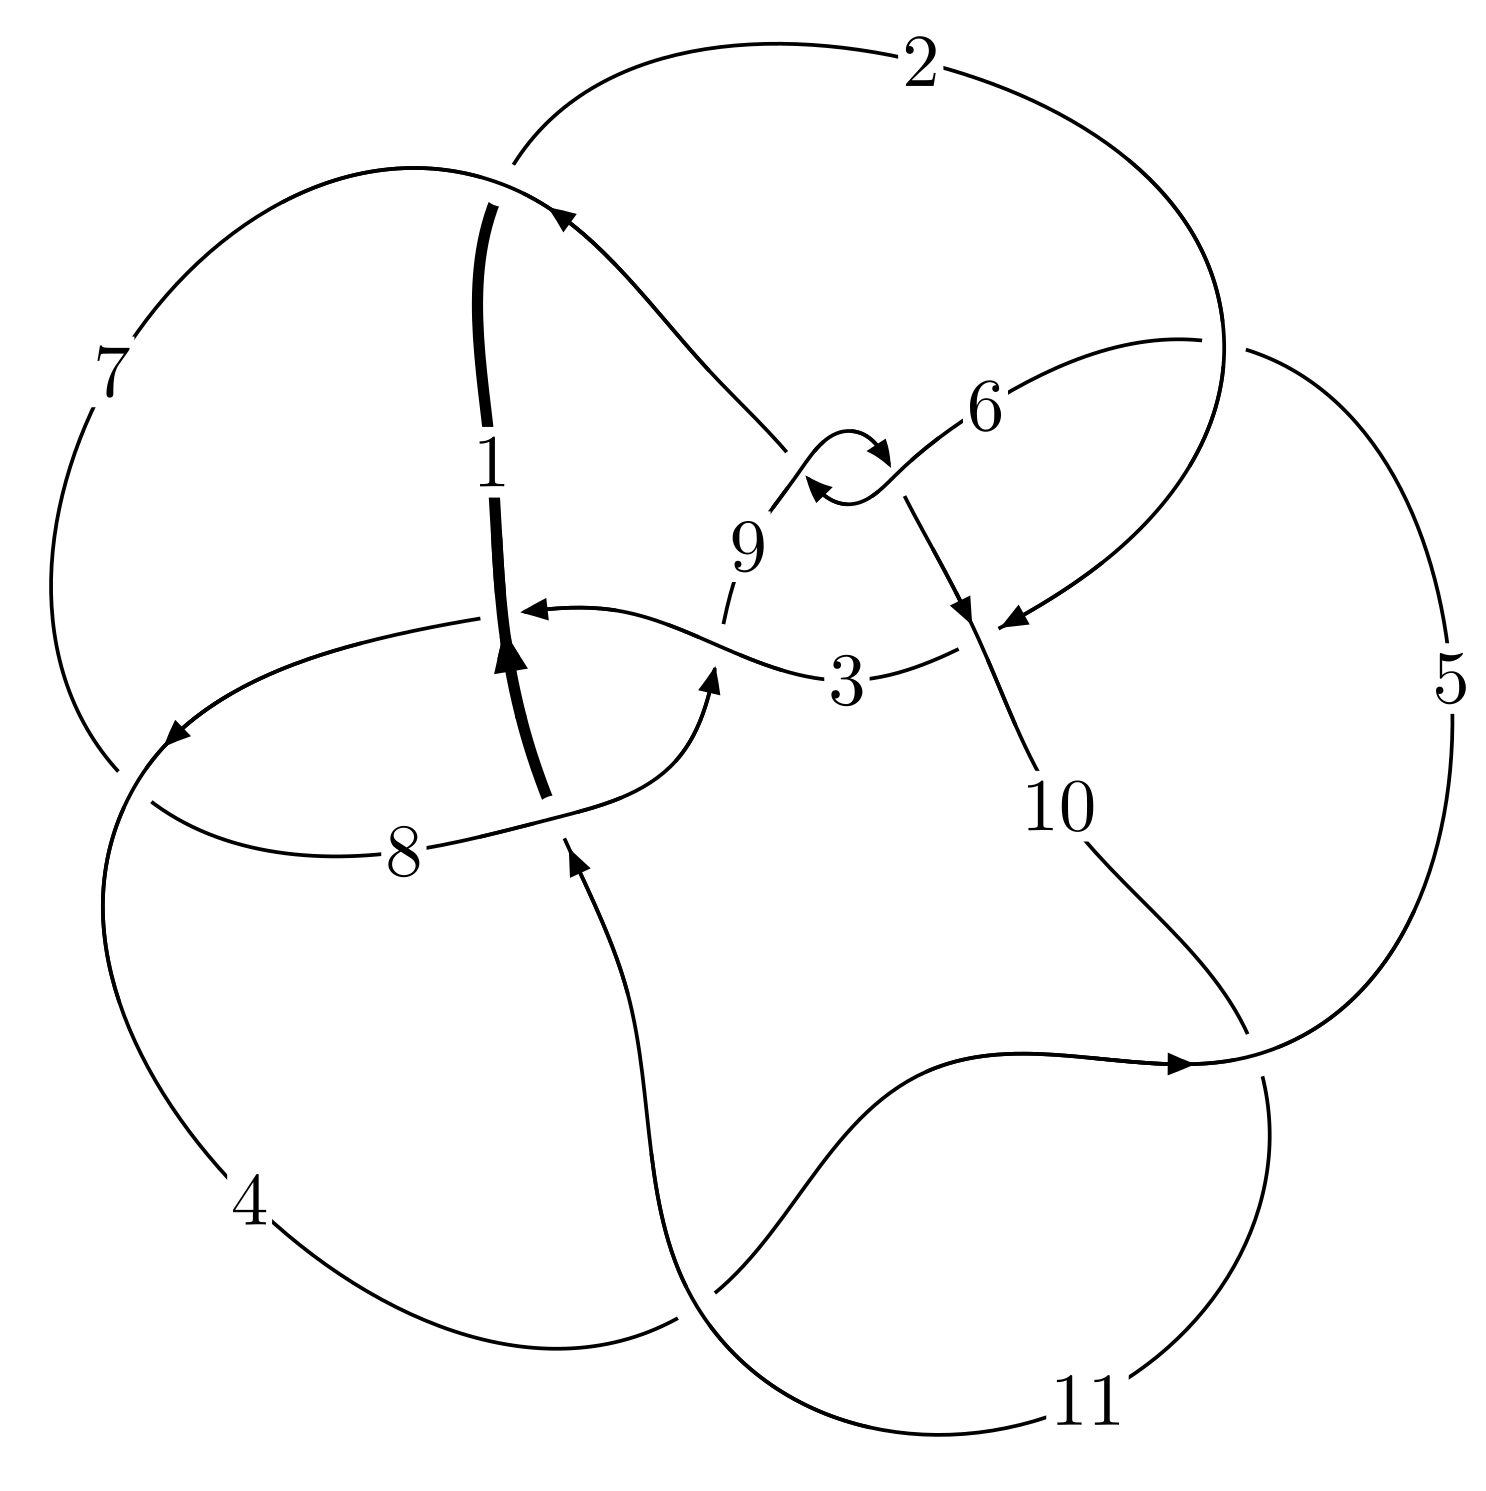
\includegraphics[width=112pt]{../../../GIT/diagram.site/Diagrams/png/534_11a_285.png}\\
\ \ \ A knot diagram\footnotemark}&
\allowdisplaybreaks
\textbf{Linearized knot diagam} \\
\cline{2-2}
 &
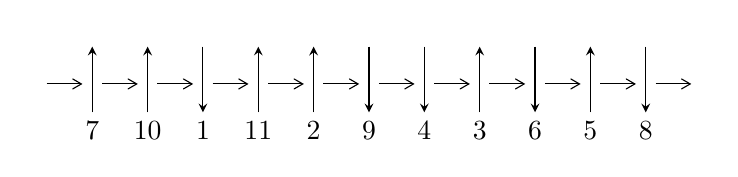
\begin{tikzpicture}[x=20pt, y=17pt]
	% nodes
	\node (C0) at (0, 0) {};
	\node (C1) at (1, 0) {};
	\node (C1U) at (1, +1) {};
	\node (C1D) at (1, -1) {7};

	\node (C2) at (2, 0) {};
	\node (C2U) at (2, +1) {};
	\node (C2D) at (2, -1) {10};

	\node (C3) at (3, 0) {};
	\node (C3U) at (3, +1) {};
	\node (C3D) at (3, -1) {1};

	\node (C4) at (4, 0) {};
	\node (C4U) at (4, +1) {};
	\node (C4D) at (4, -1) {11};

	\node (C5) at (5, 0) {};
	\node (C5U) at (5, +1) {};
	\node (C5D) at (5, -1) {2};

	\node (C6) at (6, 0) {};
	\node (C6U) at (6, +1) {};
	\node (C6D) at (6, -1) {9};

	\node (C7) at (7, 0) {};
	\node (C7U) at (7, +1) {};
	\node (C7D) at (7, -1) {4};

	\node (C8) at (8, 0) {};
	\node (C8U) at (8, +1) {};
	\node (C8D) at (8, -1) {3};

	\node (C9) at (9, 0) {};
	\node (C9U) at (9, +1) {};
	\node (C9D) at (9, -1) {6};

	\node (C10) at (10, 0) {};
	\node (C10U) at (10, +1) {};
	\node (C10D) at (10, -1) {5};

	\node (C11) at (11, 0) {};
	\node (C11U) at (11, +1) {};
	\node (C11D) at (11, -1) {8};
	\node (C12) at (12, 0) {};

	% arrows
	\draw[->,>={angle 60}]
	(C0) edge (C1) (C1) edge (C2) (C2) edge (C3) (C3) edge (C4) (C4) edge (C5) (C5) edge (C6) (C6) edge (C7) (C7) edge (C8) (C8) edge (C9) (C9) edge (C10) (C10) edge (C11) (C11) edge (C12) ;	\draw[->,>=stealth]
	(C1D) edge (C1U) (C2D) edge (C2U) (C3U) edge (C3D) (C4D) edge (C4U) (C5D) edge (C5U) (C6U) edge (C6D) (C7U) edge (C7D) (C8D) edge (C8U) (C9U) edge (C9D) (C10D) edge (C10U) (C11U) edge (C11D) ;
	\end{tikzpicture} \\
\hhline{~~} \\& 
\textbf{Solving Sequence} \\ \cline{2-2} 
 &
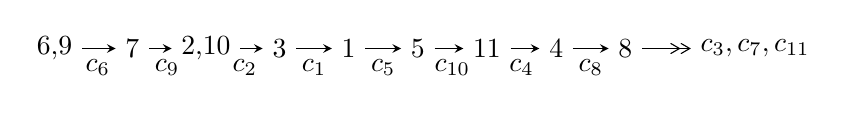
\begin{tikzpicture}[x=25pt, y=7pt]
	% node
	\node (A0) at (-1/8, 0) {6,9};
	\node (A1) at (1, 0) {7};
	\node (A2) at (33/16, 0) {2,10};
	\node (A3) at (25/8, 0) {3};
	\node (A4) at (33/8, 0) {1};
	\node (A5) at (41/8, 0) {5};
	\node (A6) at (49/8, 0) {11};
	\node (A7) at (57/8, 0) {4};
	\node (A8) at (65/8, 0) {8};
	\node (C1) at (1/2, -1) {$c_{6}$};
	\node (C2) at (3/2, -1) {$c_{9}$};
	\node (C3) at (21/8, -1) {$c_{2}$};
	\node (C4) at (29/8, -1) {$c_{1}$};
	\node (C5) at (37/8, -1) {$c_{5}$};
	\node (C6) at (45/8, -1) {$c_{10}$};
	\node (C7) at (53/8, -1) {$c_{4}$};
	\node (C8) at (61/8, -1) {$c_{8}$};
	\node (A9) at (10, 0) {$c_{3},c_{7},c_{11}$};

	% edge
	\draw[->,>=stealth]	
	(A0) edge (A1) (A1) edge (A2) (A2) edge (A3) (A3) edge (A4) (A4) edge (A5) (A5) edge (A6) (A6) edge (A7) (A7) edge (A8) ;
	\draw[->>,>={angle 60}]	
	(A8) edge (A9);
\end{tikzpicture} \\ 

\end{tabular} \\

\footnotetext{
The image of knot diagram is generated by the software ``\textbf{Draw programme}" developed by Andrew Bartholomew(\url{http://www.layer8.co.uk/maths/draw/index.htm\#Running-draw}), where we modified some parts for our purpose(\url{https://github.com/CATsTAILs/LinksPainter}).
}\phantom \\ \newline 
\centering \textbf{Ideals for irreducible components\footnotemark of $X_{\text{par}}$} 
 
\begin{align*}
I^u_{1}&=\langle 
-16908464923 u^{31}+270944948124 u^{30}+\cdots+32177743216 b+515902532096,\\
\phantom{I^u_{1}}&\phantom{= \langle  }8847487859 u^{31}-158877780023 u^{30}+\cdots+32177743216 a-2308582971600,\\
\phantom{I^u_{1}}&\phantom{= \langle  }u^{32}-16 u^{31}+\cdots-928 u+64\rangle \\
I^u_{2}&=\langle 
-3064433897 u^{10} a^5+2605872 u^{10} a^4+\cdots-83413469 a-386189933,\\
\phantom{I^u_{2}}&\phantom{= \langle  }u^{10} a^4-2 u^{10} a^3+\cdots+17 a+26,\\
\phantom{I^u_{2}}&\phantom{= \langle  }u^{11}+3 u^{10}+8 u^9+13 u^8+18 u^7+20 u^6+18 u^5+15 u^4+9 u^3+5 u^2+2 u+1\rangle \\
I^u_{3}&=\langle 
66 u^{17}-107 u^{16}+\cdots+241 b+1451,\;-1781 u^{17}+8120 u^{16}+\cdots+1205 a-4294,\\
\phantom{I^u_{3}}&\phantom{= \langle  }u^{18}-5 u^{17}+\cdots-16 u+5\rangle \\
\\
\end{align*}
\raggedright * 3 irreducible components of $\dim_{\mathbb{C}}=0$, with total 116 representations.\\
\footnotetext{All coefficients of polynomials are rational numbers. But the coefficients are sometimes approximated in decimal forms when there is not enough margin.}
\newpage
\renewcommand{\arraystretch}{1}
\centering \section*{I. $I^u_{1}= \langle -1.69\times10^{10} u^{31}+2.71\times10^{11} u^{30}+\cdots+3.22\times10^{10} b+5.16\times10^{11},\;8.85\times10^{9} u^{31}-1.59\times10^{11} u^{30}+\cdots+3.22\times10^{10} a-2.31\times10^{12},\;u^{32}-16 u^{31}+\cdots-928 u+64 \rangle$}
\flushleft \textbf{(i) Arc colorings}\\
\begin{tabular}{m{7pt} m{180pt} m{7pt} m{180pt} }
\flushright $a_{6}=$&$\begin{pmatrix}1\\0\end{pmatrix}$ \\
\flushright $a_{9}=$&$\begin{pmatrix}0\\u\end{pmatrix}$ \\
\flushright $a_{7}=$&$\begin{pmatrix}1\\u^2\end{pmatrix}$ \\
\flushright $a_{2}=$&$\begin{pmatrix}-0.274957 u^{31}+4.93751 u^{30}+\cdots-868.606 u+71.7447\\0.525471 u^{31}-8.42026 u^{30}+\cdots+288.189 u-16.0329\end{pmatrix}$ \\
\flushright $a_{10}=$&$\begin{pmatrix}- u\\u\end{pmatrix}$ \\
\flushright $a_{3}=$&$\begin{pmatrix}-0.287683 u^{31}+4.19788 u^{30}+\cdots-397.002 u+38.1146\\0.538197 u^{31}-7.68064 u^{30}+\cdots-183.415 u+17.5972\end{pmatrix}$ \\
\flushright $a_{1}=$&$\begin{pmatrix}0.130093 u^{31}-1.36022 u^{30}+\cdots-639.751 u+53.3330\\-0.139506 u^{31}+1.15527 u^{30}+\cdots+432.165 u-27.7501\end{pmatrix}$ \\
\flushright $a_{5}=$&$\begin{pmatrix}0.138364 u^{31}-2.12418 u^{30}+\cdots-252.671 u+29.4083\\-0.0517974 u^{31}+0.687312 u^{30}+\cdots+103.202 u-5.54028\end{pmatrix}$ \\
\flushright $a_{11}=$&$\begin{pmatrix}0.0893083 u^{31}-0.542520 u^{30}+\cdots-689.705 u+59.6116\\0.785648 u^{31}-12.8126 u^{30}+\cdots+866.867 u-59.3123\end{pmatrix}$ \\
\flushright $a_{4}=$&$\begin{pmatrix}-0.586797 u^{31}+9.44317 u^{30}+\cdots-913.295 u+78.7017\\1.17594 u^{31}-17.7691 u^{30}+\cdots+35.8365 u+6.83868\end{pmatrix}$ \\
\flushright $a_{8}=$&$\begin{pmatrix}-0.364711 u^{31}+5.33393 u^{30}+\cdots+228.342 u-24.1741\\0.367792 u^{31}-5.49811 u^{30}+\cdots+78.9380 u-7.54925\end{pmatrix}$\\ \flushright $a_{8}=$&$\begin{pmatrix}-0.364711 u^{31}+5.33393 u^{30}+\cdots+228.342 u-24.1741\\0.367792 u^{31}-5.49811 u^{30}+\cdots+78.9380 u-7.54925\end{pmatrix}$\\&\end{tabular}
\flushleft \textbf{(ii) Obstruction class $= -1$}\\~\\
\flushleft \textbf{(iii) Cusp Shapes $= \frac{30004216785}{8044435804} u^{31}-\frac{117366210032}{2011108951} u^{30}+\cdots+\frac{6780572708835}{2011108951} u-\frac{518436882606}{2011108951}$}\\~\\
\newpage\renewcommand{\arraystretch}{1}
\flushleft \textbf{(iv) u-Polynomials at the component}\newline \\
\begin{tabular}{m{50pt}|m{274pt}}
Crossings & \hspace{64pt}u-Polynomials at each crossing \\
\hline $$\begin{aligned}c_{1},c_{8}\end{aligned}$$&$\begin{aligned}
&u^{32}+7 u^{30}+\cdots+9 u+7
\end{aligned}$\\
\hline $$\begin{aligned}c_{2},c_{5}\end{aligned}$$&$\begin{aligned}
&u^{32}-3 u^{30}+\cdots+2 u+1
\end{aligned}$\\
\hline $$\begin{aligned}c_{3}\end{aligned}$$&$\begin{aligned}
&u^{32}-24 u^{31}+\cdots-32 u+8
\end{aligned}$\\
\hline $$\begin{aligned}c_{4},c_{10}\end{aligned}$$&$\begin{aligned}
&u^{32}-22 u^{31}+\cdots-31744 u+2048
\end{aligned}$\\
\hline $$\begin{aligned}c_{6},c_{9}\end{aligned}$$&$\begin{aligned}
&u^{32}-16 u^{31}+\cdots-928 u+64
\end{aligned}$\\
\hline $$\begin{aligned}c_{7},c_{11}\end{aligned}$$&$\begin{aligned}
&u^{32}+2 u^{31}+\cdots+u+1
\end{aligned}$\\
\hline
\end{tabular}\\~\\
\newpage\renewcommand{\arraystretch}{1}
\flushleft \textbf{(v) Riley Polynomials at the component}\newline \\
\begin{tabular}{m{50pt}|m{274pt}}
Crossings & \hspace{64pt}Riley Polynomials at each crossing \\
\hline $$\begin{aligned}c_{1},c_{8}\end{aligned}$$&$\begin{aligned}
&y^{32}+14 y^{31}+\cdots+255 y+49
\end{aligned}$\\
\hline $$\begin{aligned}c_{2},c_{5}\end{aligned}$$&$\begin{aligned}
&y^{32}-6 y^{31}+\cdots-4 y+1
\end{aligned}$\\
\hline $$\begin{aligned}c_{3}\end{aligned}$$&$\begin{aligned}
&y^{32}-6 y^{31}+\cdots-1952 y+64
\end{aligned}$\\
\hline $$\begin{aligned}c_{4},c_{10}\end{aligned}$$&$\begin{aligned}
&y^{32}+18 y^{31}+\cdots-13631488 y+4194304
\end{aligned}$\\
\hline $$\begin{aligned}c_{6},c_{9}\end{aligned}$$&$\begin{aligned}
&y^{32}+20 y^{31}+\cdots-26112 y+4096
\end{aligned}$\\
\hline $$\begin{aligned}c_{7},c_{11}\end{aligned}$$&$\begin{aligned}
&y^{32}-2 y^{31}+\cdots+7 y+1
\end{aligned}$\\
\hline
\end{tabular}\\~\\
\newpage\flushleft \textbf{(vi) Complex Volumes and Cusp Shapes}
$$\begin{array}{c|c|c}  
\text{Solutions to }I^u_{1}& \I (\text{vol} + \sqrt{-1}CS) & \text{Cusp shape}\\
 \hline 
\begin{aligned}
u &= -0.069081 + 0.991260 I \\
a &= -1.59237 - 0.40807 I \\
b &= \phantom{-}0.981760 - 0.539794 I\end{aligned}
 & \phantom{-}2.80061 + 0.23375 I & \phantom{-}8.56360 + 0. I\phantom{ +0.000000I} \\ \hline\begin{aligned}
u &= -0.069081 - 0.991260 I \\
a &= -1.59237 + 0.40807 I \\
b &= \phantom{-}0.981760 + 0.539794 I\end{aligned}
 & \phantom{-}2.80061 - 0.23375 I & \phantom{-}8.56360 + 0. I\phantom{ +0.000000I} \\ \hline\begin{aligned}
u &= \phantom{-}0.963662 + 0.325614 I \\
a &= -0.260995 + 0.288100 I \\
b &= -0.701262 - 0.982261 I\end{aligned}
 & -7.41499 + 4.16698 I & -7.97108 - 5.36120 I \\ \hline\begin{aligned}
u &= \phantom{-}0.963662 - 0.325614 I \\
a &= -0.260995 - 0.288100 I \\
b &= -0.701262 + 0.982261 I\end{aligned}
 & -7.41499 - 4.16698 I & -7.97108 + 5.36120 I \\ \hline\begin{aligned}
u &= -0.011548 + 0.974177 I \\
a &= \phantom{-}2.17659 + 0.12878 I \\
b &= -1.12385 + 1.01238 I\end{aligned}
 & -1.44736 - 2.80022 I & \phantom{-}2.50557 + 2.98682 I \\ \hline\begin{aligned}
u &= -0.011548 - 0.974177 I \\
a &= \phantom{-}2.17659 - 0.12878 I \\
b &= -1.12385 - 1.01238 I\end{aligned}
 & -1.44736 + 2.80022 I & \phantom{-}2.50557 - 2.98682 I \\ \hline\begin{aligned}
u &= -0.390961 + 1.072250 I \\
a &= \phantom{-}0.784641 + 0.086239 I \\
b &= -0.460785 + 0.225412 I\end{aligned}
 & \phantom{-}0.01128 + 2.43267 I & \phantom{-0.000000 } 0 \\ \hline\begin{aligned}
u &= -0.390961 - 1.072250 I \\
a &= \phantom{-}0.784641 - 0.086239 I \\
b &= -0.460785 - 0.225412 I\end{aligned}
 & \phantom{-}0.01128 - 2.43267 I & \phantom{-0.000000 } 0 \\ \hline\begin{aligned}
u &= \phantom{-}1.162110 + 0.060966 I \\
a &= -0.050223 - 0.185144 I \\
b &= \phantom{-}0.697927 + 1.083640 I\end{aligned}
 & -8.5372 + 12.2214 I & \phantom{-0.000000 } 0 \\ \hline\begin{aligned}
u &= \phantom{-}1.162110 - 0.060966 I \\
a &= -0.050223 + 0.185144 I \\
b &= \phantom{-}0.697927 - 1.083640 I\end{aligned}
 & -8.5372 - 12.2214 I & \phantom{-0.000000 } 0\\
 \hline 
 \end{array}$$\newpage$$\begin{array}{c|c|c}  
\text{Solutions to }I^u_{1}& \I (\text{vol} + \sqrt{-1}CS) & \text{Cusp shape}\\
 \hline 
\begin{aligned}
u &= \phantom{-}0.293991 + 1.175380 I \\
a &= -1.58096 - 0.16342 I \\
b &= \phantom{-}1.089410 - 0.886387 I\end{aligned}
 & \phantom{-}4.59065 - 3.34198 I & \phantom{-0.000000 } 0 \\ \hline\begin{aligned}
u &= \phantom{-}0.293991 - 1.175380 I \\
a &= -1.58096 + 0.16342 I \\
b &= \phantom{-}1.089410 + 0.886387 I\end{aligned}
 & \phantom{-}4.59065 + 3.34198 I & \phantom{-0.000000 } 0 \\ \hline\begin{aligned}
u &= -0.017338 + 0.774002 I \\
a &= \phantom{-}0.181918 + 1.187670 I \\
b &= -0.631219 - 0.362074 I\end{aligned}
 & -1.67497 + 2.82103 I & \phantom{-}2.81601 - 3.13394 I \\ \hline\begin{aligned}
u &= -0.017338 - 0.774002 I \\
a &= \phantom{-}0.181918 - 1.187670 I \\
b &= -0.631219 + 0.362074 I\end{aligned}
 & -1.67497 - 2.82103 I & \phantom{-}2.81601 + 3.13394 I \\ \hline\begin{aligned}
u &= \phantom{-}0.689766 + 1.084060 I \\
a &= -0.976191 - 0.334653 I \\
b &= \phantom{-}1.023330 - 0.579332 I\end{aligned}
 & \phantom{-}0.94528 - 2.67893 I & \phantom{-0.000000 } 0 \\ \hline\begin{aligned}
u &= \phantom{-}0.689766 - 1.084060 I \\
a &= -0.976191 + 0.334653 I \\
b &= \phantom{-}1.023330 + 0.579332 I\end{aligned}
 & \phantom{-}0.94528 + 2.67893 I & \phantom{-0.000000 } 0 \\ \hline\begin{aligned}
u &= \phantom{-}0.568936 + 1.193230 I \\
a &= \phantom{-}1.59592 - 0.00124 I \\
b &= -1.16760 + 1.18399 I\end{aligned}
 & -4.66339 - 9.68262 I & \phantom{-0.000000 } 0 \\ \hline\begin{aligned}
u &= \phantom{-}0.568936 - 1.193230 I \\
a &= \phantom{-}1.59592 + 0.00124 I \\
b &= -1.16760 - 1.18399 I\end{aligned}
 & -4.66339 + 9.68262 I & \phantom{-0.000000 } 0 \\ \hline\begin{aligned}
u &= \phantom{-}0.215422 + 1.325080 I \\
a &= \phantom{-}1.087280 + 0.231048 I \\
b &= -0.856658 + 0.452941 I\end{aligned}
 & \phantom{-}5.14597 + 1.67947 I & \phantom{-0.000000 } 0 \\ \hline\begin{aligned}
u &= \phantom{-}0.215422 - 1.325080 I \\
a &= \phantom{-}1.087280 - 0.231048 I \\
b &= -0.856658 - 0.452941 I\end{aligned}
 & \phantom{-}5.14597 - 1.67947 I & \phantom{-0.000000 } 0\\
 \hline 
 \end{array}$$\newpage$$\begin{array}{c|c|c}  
\text{Solutions to }I^u_{1}& \I (\text{vol} + \sqrt{-1}CS) & \text{Cusp shape}\\
 \hline 
\begin{aligned}
u &= \phantom{-}1.380870 + 0.268452 I \\
a &= \phantom{-}0.081994 + 0.203286 I \\
b &= -0.477164 - 0.458499 I\end{aligned}
 & -1.75461 + 5.81807 I & \phantom{-0.000000 } 0 \\ \hline\begin{aligned}
u &= \phantom{-}1.380870 - 0.268452 I \\
a &= \phantom{-}0.081994 - 0.203286 I \\
b &= -0.477164 + 0.458499 I\end{aligned}
 & -1.75461 - 5.81807 I & \phantom{-0.000000 } 0 \\ \hline\begin{aligned}
u &= \phantom{-}0.58508 + 1.34607 I \\
a &= -1.62335 + 0.16272 I \\
b &= \phantom{-}1.17347 - 1.23003 I\end{aligned}
 & -4.5311 - 18.3328 I & \phantom{-0.000000 } 0 \\ \hline\begin{aligned}
u &= \phantom{-}0.58508 - 1.34607 I \\
a &= -1.62335 - 0.16272 I \\
b &= \phantom{-}1.17347 + 1.23003 I\end{aligned}
 & -4.5311 + 18.3328 I & \phantom{-0.000000 } 0 \\ \hline\begin{aligned}
u &= \phantom{-}0.63966 + 1.32722 I \\
a &= \phantom{-}1.276940 + 0.097523 I \\
b &= -1.102100 + 0.817123 I\end{aligned}
 & \phantom{-}1.78578 - 12.54500 I & \phantom{-0.000000 } 0 \\ \hline\begin{aligned}
u &= \phantom{-}0.63966 - 1.32722 I \\
a &= \phantom{-}1.276940 - 0.097523 I \\
b &= -1.102100 - 0.817123 I\end{aligned}
 & \phantom{-}1.78578 + 12.54500 I & \phantom{-0.000000 } 0 \\ \hline\begin{aligned}
u &= \phantom{-}0.91660 + 1.20168 I \\
a &= -0.567740 - 0.360034 I \\
b &= \phantom{-}0.833279 - 0.130849 I\end{aligned}
 & \phantom{-}0.68711 - 4.21425 I & \phantom{-0.000000 } 0 \\ \hline\begin{aligned}
u &= \phantom{-}0.91660 - 1.20168 I \\
a &= -0.567740 + 0.360034 I \\
b &= \phantom{-}0.833279 + 0.130849 I\end{aligned}
 & \phantom{-}0.68711 + 4.21425 I & \phantom{-0.000000 } 0 \\ \hline\begin{aligned}
u &= \phantom{-}0.326786 + 0.069422 I \\
a &= \phantom{-}0.97596 - 1.03690 I \\
b &= \phantom{-}0.615647 - 0.339196 I\end{aligned}
 & \phantom{-}1.110970 - 0.707958 I & \phantom{-}6.93245 + 3.29648 I \\ \hline\begin{aligned}
u &= \phantom{-}0.326786 - 0.069422 I \\
a &= \phantom{-}0.97596 + 1.03690 I \\
b &= \phantom{-}0.615647 + 0.339196 I\end{aligned}
 & \phantom{-}1.110970 + 0.707958 I & \phantom{-}6.93245 - 3.29648 I\\
 \hline 
 \end{array}$$\newpage$$\begin{array}{c|c|c}  
\text{Solutions to }I^u_{1}& \I (\text{vol} + \sqrt{-1}CS) & \text{Cusp shape}\\
 \hline 
\begin{aligned}
u &= \phantom{-}0.74605 + 1.70600 I \\
a &= \phantom{-}0.115579 - 0.368848 I \\
b &= \phantom{-}0.105807 + 0.403642 I\end{aligned}
 & -3.50340 + 5.56191 I & \phantom{-0.000000 } 0 \\ \hline\begin{aligned}
u &= \phantom{-}0.74605 - 1.70600 I \\
a &= \phantom{-}0.115579 + 0.368848 I \\
b &= \phantom{-}0.105807 - 0.403642 I\end{aligned}
 & -3.50340 - 5.56191 I & \phantom{-0.000000 } 0\\
 \hline 
 \end{array}$$\newpage\newpage\renewcommand{\arraystretch}{1}
\centering \section*{II. $I^u_{2}= \langle -3.06\times10^{9} a^{5} u^{10}+2.61\times10^{6} a^{4} u^{10}+\cdots-8.34\times10^{7} a-3.86\times10^{8},\;u^{10} a^4-2 u^{10} a^3+\cdots+17 a+26,\;u^{11}+3 u^{10}+\cdots+2 u+1 \rangle$}
\flushleft \textbf{(i) Arc colorings}\\
\begin{tabular}{m{7pt} m{180pt} m{7pt} m{180pt} }
\flushright $a_{6}=$&$\begin{pmatrix}1\\0\end{pmatrix}$ \\
\flushright $a_{9}=$&$\begin{pmatrix}0\\u\end{pmatrix}$ \\
\flushright $a_{7}=$&$\begin{pmatrix}1\\u^2\end{pmatrix}$ \\
\flushright $a_{2}=$&$\begin{pmatrix}a\\15.4325 a^{5} u^{10}-0.0131231 a^{4} u^{10}+\cdots+0.420069 a+1.94485\end{pmatrix}$ \\
\flushright $a_{10}=$&$\begin{pmatrix}- u\\u\end{pmatrix}$ \\
\flushright $a_{3}=$&$\begin{pmatrix}18.7665 a^{5} u^{10}-0.397589 a^{4} u^{10}+\cdots+1.28801 a-0.233448\\-3.33405 a^{5} u^{10}+0.384466 a^{4} u^{10}+\cdots+0.132055 a+2.17830\end{pmatrix}$ \\
\flushright $a_{1}=$&$\begin{pmatrix}-15.4325 a^{5} u^{10}+0.0131231 a^{4} u^{10}+\cdots+0.579931 a-1.94485\\-3.33405 a^{5} u^{10}+0.384466 a^{4} u^{10}+\cdots+0.132055 a+2.17830\end{pmatrix}$ \\
\flushright $a_{5}=$&$\begin{pmatrix}-9.34723 a^{5} u^{10}-4.17923 a^{4} u^{10}+\cdots-1.73376 a+3.01241\\-11.6963 a^{5} u^{10}-5.05510 a^{4} u^{10}+\cdots+0.553825 a-1.80148\end{pmatrix}$ \\
\flushright $a_{11}=$&$\begin{pmatrix}27.6580 a^{5} u^{10}+14.2554 a^{4} u^{10}+\cdots-0.232159 a-1.97655\\-11.2026 a^{5} u^{10}-4.82036 a^{4} u^{10}+\cdots-1.18924 a+2.53573\end{pmatrix}$ \\
\flushright $a_{4}=$&$\begin{pmatrix}10.1325 a^{5} u^{10}-0.446147 a^{4} u^{10}+\cdots+0.381091 a+2.69045\\-5.54424 a^{5} u^{10}+0.245395 a^{4} u^{10}+\cdots+2.22025 a-2.46057\end{pmatrix}$ \\
\flushright $a_{8}=$&$\begin{pmatrix}-77.2129 a^{5} u^{10}-33.1153 a^{4} u^{10}+\cdots-0.660872 a-0.00581236\\24.7170 a^{5} u^{10}+10.4299 a^{4} u^{10}+\cdots+0.680370 a+0.715387\end{pmatrix}$\\ \flushright $a_{8}=$&$\begin{pmatrix}-77.2129 a^{5} u^{10}-33.1153 a^{4} u^{10}+\cdots-0.660872 a-0.00581236\\24.7170 a^{5} u^{10}+10.4299 a^{4} u^{10}+\cdots+0.680370 a+0.715387\end{pmatrix}$\\&\end{tabular}
\flushleft \textbf{(ii) Obstruction class $= -1$}\\~\\
\flushleft \textbf{(iii) Cusp Shapes $= \frac{4036276680}{198570719} u^{10} a^5-\frac{180111700}{198570719} u^{10} a^4+\cdots+\frac{284371904}{198570719} a-\frac{303474202}{198570719}$}\\~\\
\newpage\renewcommand{\arraystretch}{1}
\flushleft \textbf{(iv) u-Polynomials at the component}\newline \\
\begin{tabular}{m{50pt}|m{274pt}}
Crossings & \hspace{64pt}u-Polynomials at each crossing \\
\hline $$\begin{aligned}c_{1},c_{8}\end{aligned}$$&$\begin{aligned}
&u^{66}+u^{65}+\cdots+345266 u+66193
\end{aligned}$\\
\hline $$\begin{aligned}c_{2},c_{5}\end{aligned}$$&$\begin{aligned}
&u^{66}- u^{65}+\cdots+30 u+1
\end{aligned}$\\
\hline $$\begin{aligned}c_{3}\end{aligned}$$&$\begin{aligned}
&(u^{11}+5 u^{10}+12 u^9+15 u^8+8 u^7-4 u^6-8 u^5-3 u^4+3 u^3+3 u^2-1)^6
\end{aligned}$\\
\hline $$\begin{aligned}c_{4},c_{10}\end{aligned}$$&$\begin{aligned}
&(u^3+u^2+2 u+1)^{22}
\end{aligned}$\\
\hline $$\begin{aligned}c_{6},c_{9}\end{aligned}$$&$\begin{aligned}
&(u^{11}+3 u^{10}+\cdots+2 u+1)^{6}
\end{aligned}$\\
\hline $$\begin{aligned}c_{7},c_{11}\end{aligned}$$&$\begin{aligned}
&u^{66}+3 u^{65}+\cdots+2656 u+691
\end{aligned}$\\
\hline
\end{tabular}\\~\\
\newpage\renewcommand{\arraystretch}{1}
\flushleft \textbf{(v) Riley Polynomials at the component}\newline \\
\begin{tabular}{m{50pt}|m{274pt}}
Crossings & \hspace{64pt}Riley Polynomials at each crossing \\
\hline $$\begin{aligned}c_{1},c_{8}\end{aligned}$$&$\begin{aligned}
&y^{66}+27 y^{65}+\cdots+109594377816 y+4381513249
\end{aligned}$\\
\hline $$\begin{aligned}c_{2},c_{5}\end{aligned}$$&$\begin{aligned}
&y^{66}+15 y^{65}+\cdots-104 y+1
\end{aligned}$\\
\hline $$\begin{aligned}c_{3}\end{aligned}$$&$\begin{aligned}
&(y^{11}- y^{10}+\cdots+6 y-1)^{6}
\end{aligned}$\\
\hline $$\begin{aligned}c_{4},c_{10}\end{aligned}$$&$\begin{aligned}
&(y^3+3 y^2+2 y-1)^{22}
\end{aligned}$\\
\hline $$\begin{aligned}c_{6},c_{9}\end{aligned}$$&$\begin{aligned}
&(y^{11}+7 y^{10}+\cdots-6 y-1)^{6}
\end{aligned}$\\
\hline $$\begin{aligned}c_{7},c_{11}\end{aligned}$$&$\begin{aligned}
&y^{66}-25 y^{65}+\cdots-19619480 y+477481
\end{aligned}$\\
\hline
\end{tabular}\\~\\
\newpage\flushleft \textbf{(vi) Complex Volumes and Cusp Shapes}
$$\begin{array}{c|c|c}  
\text{Solutions to }I^u_{2}& \I (\text{vol} + \sqrt{-1}CS) & \text{Cusp shape}\\
 \hline 
\begin{aligned}
u &= \phantom{-}0.253759 + 0.946686 I \\
a &= \phantom{-}0.665253 + 0.858657 I \\
b &= -0.283695 + 1.126660 I\end{aligned}
 & -4.53141 - 2.38817 I & -3.94579 + 6.03333 I \\ \hline\begin{aligned}
u &= \phantom{-}0.253759 + 0.946686 I \\
a &= \phantom{-}0.400243 + 0.809909 I \\
b &= -0.50925 - 1.57544 I\end{aligned}
 & -0.39383 - 5.21629 I & \phantom{-}2.58348 + 9.01278 I \\ \hline\begin{aligned}
u &= \phantom{-}0.253759 + 0.946686 I \\
a &= -2.38419 + 0.38315 I \\
b &= \phantom{-}0.697054 - 0.297456 I\end{aligned}
 & -0.39383 - 5.21629 I & \phantom{-}2.58348 + 9.01278 I \\ \hline\begin{aligned}
u &= \phantom{-}0.253759 + 0.946686 I \\
a &= -1.41166 - 2.08569 I \\
b &= \phantom{-}1.62854 + 2.14254 I\end{aligned}
 & -4.53141 - 8.04441 I & -3.94579 + 11.99222 I \\ \hline\begin{aligned}
u &= \phantom{-}0.253759 + 0.946686 I \\
a &= \phantom{-}2.81803 - 0.28780 I \\
b &= -1.78265 + 0.86501 I\end{aligned}
 & -4.53141 - 2.38817 I & -3.94579 + 6.03333 I \\ \hline\begin{aligned}
u &= \phantom{-}0.253759 + 0.946686 I \\
a &= \phantom{-}2.54048 - 1.25869 I \\
b &= \phantom{-}0.001211 + 0.219744 I\end{aligned}
 & -4.53141 - 8.04441 I & -3.94579 + 11.99222 I \\ \hline\begin{aligned}
u &= \phantom{-}0.253759 - 0.946686 I \\
a &= \phantom{-}0.665253 - 0.858657 I \\
b &= -0.283695 - 1.126660 I\end{aligned}
 & -4.53141 + 2.38817 I & -3.94579 - 6.03333 I \\ \hline\begin{aligned}
u &= \phantom{-}0.253759 - 0.946686 I \\
a &= \phantom{-}0.400243 - 0.809909 I \\
b &= -0.50925 + 1.57544 I\end{aligned}
 & -0.39383 + 5.21629 I & \phantom{-}2.58348 - 9.01278 I \\ \hline\begin{aligned}
u &= \phantom{-}0.253759 - 0.946686 I \\
a &= -2.38419 - 0.38315 I \\
b &= \phantom{-}0.697054 + 0.297456 I\end{aligned}
 & -0.39383 + 5.21629 I & \phantom{-}2.58348 - 9.01278 I \\ \hline\begin{aligned}
u &= \phantom{-}0.253759 - 0.946686 I \\
a &= -1.41166 + 2.08569 I \\
b &= \phantom{-}1.62854 - 2.14254 I\end{aligned}
 & -4.53141 + 8.04441 I & -3.94579 - 11.99222 I\\
 \hline 
 \end{array}$$\newpage$$\begin{array}{c|c|c}  
\text{Solutions to }I^u_{2}& \I (\text{vol} + \sqrt{-1}CS) & \text{Cusp shape}\\
 \hline 
\begin{aligned}
u &= \phantom{-}0.253759 - 0.946686 I \\
a &= \phantom{-}2.81803 + 0.28780 I \\
b &= -1.78265 - 0.86501 I\end{aligned}
 & -4.53141 + 2.38817 I & -3.94579 - 6.03333 I \\ \hline\begin{aligned}
u &= \phantom{-}0.253759 - 0.946686 I \\
a &= \phantom{-}2.54048 + 1.25869 I \\
b &= \phantom{-}0.001211 - 0.219744 I\end{aligned}
 & -4.53141 + 8.04441 I & -3.94579 - 11.99222 I \\ \hline\begin{aligned}
u &= -1.10821\phantom{ +0.000000I} \\
a &= -0.326400 + 0.336410 I \\
b &= \phantom{-}0.74092 - 1.23654 I\end{aligned}
 & -7.04782 - 2.82812 I & -15.7711 + 2.9794 I \\ \hline\begin{aligned}
u &= -1.10821\phantom{ +0.000000I} \\
a &= -0.326400 - 0.336410 I \\
b &= \phantom{-}0.74092 + 1.23654 I\end{aligned}
 & -7.04782 + 2.82812 I & -15.7711 - 2.9794 I \\ \hline\begin{aligned}
u &= -1.10821\phantom{ +0.000000I} \\
a &= \phantom{-}0.230392 + 0.070664 I \\
b &= -0.121109 - 0.723675 I\end{aligned}
 & -2.91024\phantom{ +0.000000I} & -9.24183 + 0. I\phantom{ +0.000000I} \\ \hline\begin{aligned}
u &= -1.10821\phantom{ +0.000000I} \\
a &= \phantom{-}0.230392 - 0.070664 I \\
b &= -0.121109 + 0.723675 I\end{aligned}
 & -2.91024\phantom{ +0.000000I} & -9.24183 + 0. I\phantom{ +0.000000I} \\ \hline\begin{aligned}
u &= -1.10821\phantom{ +0.000000I} \\
a &= -0.209195 + 0.118260 I \\
b &= -0.459379 + 0.997538 I\end{aligned}
 & -7.04782 - 2.82812 I & -15.7711 + 2.9794 I \\ \hline\begin{aligned}
u &= -1.10821\phantom{ +0.000000I} \\
a &= -0.209195 - 0.118260 I \\
b &= -0.459379 - 0.997538 I\end{aligned}
 & -7.04782 + 2.82812 I & -15.7711 - 2.9794 I \\ \hline\begin{aligned}
u &= -0.572881 + 0.536287 I \\
a &= -0.178622 - 0.995404 I \\
b &= -0.391403 - 1.054420 I\end{aligned}
 & -5.09306 + 5.07591 I & -7.14557 - 8.04304 I \\ \hline\begin{aligned}
u &= -0.572881 + 0.536287 I \\
a &= \phantom{-}1.097050 - 0.676541 I \\
b &= -0.663433 - 0.206361 I\end{aligned}
 & -0.95548 + 2.24779 I & -0.61631 - 5.06360 I\\
 \hline 
 \end{array}$$\newpage$$\begin{array}{c|c|c}  
\text{Solutions to }I^u_{2}& \I (\text{vol} + \sqrt{-1}CS) & \text{Cusp shape}\\
 \hline 
\begin{aligned}
u &= -0.572881 + 0.536287 I \\
a &= -1.198410 + 0.589737 I \\
b &= -0.430728 + 0.376103 I\end{aligned}
 & -5.09306 - 0.58034 I & -7.14557 - 2.08415 I \\ \hline\begin{aligned}
u &= -0.572881 + 0.536287 I \\
a &= \phantom{-}0.31292 + 1.45222 I \\
b &= \phantom{-}0.41533 - 1.42699 I\end{aligned}
 & -5.09306 - 0.58034 I & -7.14557 - 2.08415 I \\ \hline\begin{aligned}
u &= -0.572881 + 0.536287 I \\
a &= \phantom{-}0.212405 + 0.031411 I \\
b &= \phantom{-}0.225077 + 0.738341 I\end{aligned}
 & -0.95548 + 2.24779 I & -0.61631 - 5.06360 I \\ \hline\begin{aligned}
u &= -0.572881 + 0.536287 I \\
a &= -1.98001 + 0.45319 I \\
b &= \phantom{-}1.42585 + 0.86861 I\end{aligned}
 & -5.09306 + 5.07591 I & -7.14557 - 8.04304 I \\ \hline\begin{aligned}
u &= -0.572881 - 0.536287 I \\
a &= -0.178622 + 0.995404 I \\
b &= -0.391403 + 1.054420 I\end{aligned}
 & -5.09306 - 5.07591 I & -7.14557 + 8.04304 I \\ \hline\begin{aligned}
u &= -0.572881 - 0.536287 I \\
a &= \phantom{-}1.097050 + 0.676541 I \\
b &= -0.663433 + 0.206361 I\end{aligned}
 & -0.95548 - 2.24779 I & -0.61631 + 5.06360 I \\ \hline\begin{aligned}
u &= -0.572881 - 0.536287 I \\
a &= -1.198410 - 0.589737 I \\
b &= -0.430728 - 0.376103 I\end{aligned}
 & -5.09306 + 0.58034 I & -7.14557 + 2.08415 I \\ \hline\begin{aligned}
u &= -0.572881 - 0.536287 I \\
a &= \phantom{-}0.31292 - 1.45222 I \\
b &= \phantom{-}0.41533 + 1.42699 I\end{aligned}
 & -5.09306 + 0.58034 I & -7.14557 + 2.08415 I \\ \hline\begin{aligned}
u &= -0.572881 - 0.536287 I \\
a &= \phantom{-}0.212405 - 0.031411 I \\
b &= \phantom{-}0.225077 - 0.738341 I\end{aligned}
 & -0.95548 - 2.24779 I & -0.61631 + 5.06360 I \\ \hline\begin{aligned}
u &= -0.572881 - 0.536287 I \\
a &= -1.98001 - 0.45319 I \\
b &= \phantom{-}1.42585 - 0.86861 I\end{aligned}
 & -5.09306 - 5.07591 I & -7.14557 + 8.04304 I\\
 \hline 
 \end{array}$$\newpage$$\begin{array}{c|c|c}  
\text{Solutions to }I^u_{2}& \I (\text{vol} + \sqrt{-1}CS) & \text{Cusp shape}\\
 \hline 
\begin{aligned}
u &= -0.290349 + 1.272230 I \\
a &= \phantom{-}1.001860 + 0.001395 I \\
b &= -1.018330 + 0.058723 I\end{aligned}
 & -0.03833 + 2.17262 I & \phantom{-}4.33084 - 3.24807 I \\ \hline\begin{aligned}
u &= -0.290349 + 1.272230 I \\
a &= \phantom{-}0.289202 + 0.789207 I \\
b &= -0.0716992 - 0.0384158 I\end{aligned}
 & -0.03833 + 2.17262 I & \phantom{-}4.33084 - 3.24807 I \\ \hline\begin{aligned}
u &= -0.290349 + 1.272230 I \\
a &= \phantom{-}1.178120 - 0.545316 I \\
b &= -0.654660 - 0.523893 I\end{aligned}
 & \phantom{-}4.09925 + 5.00074 I & \phantom{-}10.86010 - 6.22751 I \\ \hline\begin{aligned}
u &= -0.290349 + 1.272230 I \\
a &= -1.48808 - 0.39798 I \\
b &= \phantom{-}1.20830 + 0.97641 I\end{aligned}
 & \phantom{-}4.09925 + 5.00074 I & \phantom{-}10.86010 - 6.22751 I \\ \hline\begin{aligned}
u &= -0.290349 + 1.272230 I \\
a &= \phantom{-}1.53917 + 0.91664 I \\
b &= -1.18366 - 1.77329 I\end{aligned}
 & -0.03833 + 7.82886 I & \phantom{-}4.33084 - 9.20696 I \\ \hline\begin{aligned}
u &= -0.290349 + 1.272230 I \\
a &= -2.10966 + 0.48565 I \\
b &= \phantom{-}0.986642 + 0.701021 I\end{aligned}
 & -0.03833 + 7.82886 I & \phantom{-}4.33084 - 9.20696 I \\ \hline\begin{aligned}
u &= -0.290349 - 1.272230 I \\
a &= \phantom{-}1.001860 - 0.001395 I \\
b &= -1.018330 - 0.058723 I\end{aligned}
 & -0.03833 - 2.17262 I & \phantom{-}4.33084 + 3.24807 I \\ \hline\begin{aligned}
u &= -0.290349 - 1.272230 I \\
a &= \phantom{-}0.289202 - 0.789207 I \\
b &= -0.0716992 + 0.0384158 I\end{aligned}
 & -0.03833 - 2.17262 I & \phantom{-}4.33084 + 3.24807 I \\ \hline\begin{aligned}
u &= -0.290349 - 1.272230 I \\
a &= \phantom{-}1.178120 + 0.545316 I \\
b &= -0.654660 + 0.523893 I\end{aligned}
 & \phantom{-}4.09925 - 5.00074 I & \phantom{-}10.86010 + 6.22751 I \\ \hline\begin{aligned}
u &= -0.290349 - 1.272230 I \\
a &= -1.48808 + 0.39798 I \\
b &= \phantom{-}1.20830 - 0.97641 I\end{aligned}
 & \phantom{-}4.09925 - 5.00074 I & \phantom{-}10.86010 + 6.22751 I\\
 \hline 
 \end{array}$$\newpage$$\begin{array}{c|c|c}  
\text{Solutions to }I^u_{2}& \I (\text{vol} + \sqrt{-1}CS) & \text{Cusp shape}\\
 \hline 
\begin{aligned}
u &= -0.290349 - 1.272230 I \\
a &= \phantom{-}1.53917 - 0.91664 I \\
b &= -1.18366 + 1.77329 I\end{aligned}
 & -0.03833 - 7.82886 I & \phantom{-}4.33084 + 9.20696 I \\ \hline\begin{aligned}
u &= -0.290349 - 1.272230 I \\
a &= -2.10966 - 0.48565 I \\
b &= \phantom{-}0.986642 - 0.701021 I\end{aligned}
 & -0.03833 - 7.82886 I & \phantom{-}4.33084 + 9.20696 I \\ \hline\begin{aligned}
u &= \phantom{-}0.234018 + 0.605151 I \\
a &= -0.239136 + 0.416643 I \\
b &= \phantom{-}0.439230 + 0.995032 I\end{aligned}
 & -1.33438 + 2.70441 I & -0.448108 + 0.083327 I \\ \hline\begin{aligned}
u &= \phantom{-}0.234018 + 0.605151 I \\
a &= \phantom{-}0.06031 + 1.80790 I \\
b &= -0.74955 - 1.66176 I\end{aligned}
 & -5.47196 - 0.12371 I & -6.97737 + 3.06277 I \\ \hline\begin{aligned}
u &= \phantom{-}0.234018 + 0.605151 I \\
a &= \phantom{-}0.68960 - 1.93675 I \\
b &= -0.069788 - 1.004720 I\end{aligned}
 & -5.47196 + 5.53253 I & -6.97737 - 2.89612 I \\ \hline\begin{aligned}
u &= \phantom{-}0.234018 + 0.605151 I \\
a &= \phantom{-}2.48198 - 0.52970 I \\
b &= -0.807451 + 0.451445 I\end{aligned}
 & -1.33438 + 2.70441 I & -0.448108 + 0.083327 I \\ \hline\begin{aligned}
u &= \phantom{-}0.234018 + 0.605151 I \\
a &= -2.55575 + 0.53661 I \\
b &= -0.249729 - 0.382896 I\end{aligned}
 & -5.47196 - 0.12371 I & -6.97737 + 3.06277 I \\ \hline\begin{aligned}
u &= \phantom{-}0.234018 + 0.605151 I \\
a &= -3.40816 - 0.14493 I \\
b &= \phantom{-}1.92508 - 0.31327 I\end{aligned}
 & -5.47196 + 5.53253 I & -6.97737 - 2.89612 I \\ \hline\begin{aligned}
u &= \phantom{-}0.234018 - 0.605151 I \\
a &= -0.239136 - 0.416643 I \\
b &= \phantom{-}0.439230 - 0.995032 I\end{aligned}
 & -1.33438 - 2.70441 I & -0.448108 - 0.083327 I \\ \hline\begin{aligned}
u &= \phantom{-}0.234018 - 0.605151 I \\
a &= \phantom{-}0.06031 - 1.80790 I \\
b &= -0.74955 + 1.66176 I\end{aligned}
 & -5.47196 + 0.12371 I & -6.97737 - 3.06277 I\\
 \hline 
 \end{array}$$\newpage$$\begin{array}{c|c|c}  
\text{Solutions to }I^u_{2}& \I (\text{vol} + \sqrt{-1}CS) & \text{Cusp shape}\\
 \hline 
\begin{aligned}
u &= \phantom{-}0.234018 - 0.605151 I \\
a &= \phantom{-}0.68960 + 1.93675 I \\
b &= -0.069788 + 1.004720 I\end{aligned}
 & -5.47196 - 5.53253 I & -6.97737 + 2.89612 I \\ \hline\begin{aligned}
u &= \phantom{-}0.234018 - 0.605151 I \\
a &= \phantom{-}2.48198 + 0.52970 I \\
b &= -0.807451 - 0.451445 I\end{aligned}
 & -1.33438 - 2.70441 I & -0.448108 - 0.083327 I \\ \hline\begin{aligned}
u &= \phantom{-}0.234018 - 0.605151 I \\
a &= -2.55575 - 0.53661 I \\
b &= -0.249729 + 0.382896 I\end{aligned}
 & -5.47196 + 0.12371 I & -6.97737 - 3.06277 I \\ \hline\begin{aligned}
u &= \phantom{-}0.234018 - 0.605151 I \\
a &= -3.40816 + 0.14493 I \\
b &= \phantom{-}1.92508 + 0.31327 I\end{aligned}
 & -5.47196 - 5.53253 I & -6.97737 + 2.89612 I \\ \hline\begin{aligned}
u &= -0.57044 + 1.34258 I \\
a &= -0.907349 - 0.181245 I \\
b &= \phantom{-}0.714414 + 0.937746 I\end{aligned}
 & \phantom{-}1.22875 + 5.92443 I & -0.15094 - 10.02355 I \\ \hline\begin{aligned}
u &= -0.57044 + 1.34258 I \\
a &= \phantom{-}0.292115 + 0.758984 I \\
b &= -0.042421 - 0.880536 I\end{aligned}
 & -2.90883 + 3.09630 I & -6.68021 - 7.04410 I \\ \hline\begin{aligned}
u &= -0.57044 + 1.34258 I \\
a &= \phantom{-}1.231120 + 0.121507 I \\
b &= -0.84877 - 1.26334 I\end{aligned}
 & -2.90883 + 8.75255 I & -6.6802 - 13.0030 I \\ \hline\begin{aligned}
u &= -0.57044 + 1.34258 I \\
a &= \phantom{-}1.305750 - 0.011564 I \\
b &= -0.905606 - 0.690569 I\end{aligned}
 & \phantom{-}1.22875 + 5.92443 I & -0.15094 - 10.02355 I \\ \hline\begin{aligned}
u &= -0.57044 + 1.34258 I \\
a &= -0.564946 - 0.141760 I \\
b &= \phantom{-}0.020758 + 0.404573 I\end{aligned}
 & -2.90883 + 3.09630 I & -6.68021 - 7.04410 I \\ \hline\begin{aligned}
u &= -0.57044 + 1.34258 I \\
a &= -1.88445 - 0.29051 I \\
b &= \phantom{-}1.31490 + 1.16469 I\end{aligned}
 & -2.90883 + 8.75255 I & -6.6802 - 13.0030 I\\
 \hline 
 \end{array}$$\newpage$$\begin{array}{c|c|c}  
\text{Solutions to }I^u_{2}& \I (\text{vol} + \sqrt{-1}CS) & \text{Cusp shape}\\
 \hline 
\begin{aligned}
u &= -0.57044 - 1.34258 I \\
a &= -0.907349 + 0.181245 I \\
b &= \phantom{-}0.714414 - 0.937746 I\end{aligned}
 & \phantom{-}1.22875 - 5.92443 I & -0.15094 + 10.02355 I \\ \hline\begin{aligned}
u &= -0.57044 - 1.34258 I \\
a &= \phantom{-}0.292115 - 0.758984 I \\
b &= -0.042421 + 0.880536 I\end{aligned}
 & -2.90883 - 3.09630 I & -6.68021 + 7.04410 I \\ \hline\begin{aligned}
u &= -0.57044 - 1.34258 I \\
a &= \phantom{-}1.231120 - 0.121507 I \\
b &= -0.84877 + 1.26334 I\end{aligned}
 & -2.90883 - 8.75255 I & -6.6802 + 13.0030 I \\ \hline\begin{aligned}
u &= -0.57044 - 1.34258 I \\
a &= \phantom{-}1.305750 + 0.011564 I \\
b &= -0.905606 + 0.690569 I\end{aligned}
 & \phantom{-}1.22875 - 5.92443 I & -0.15094 + 10.02355 I \\ \hline\begin{aligned}
u &= -0.57044 - 1.34258 I \\
a &= -0.564946 + 0.141760 I \\
b &= \phantom{-}0.020758 - 0.404573 I\end{aligned}
 & -2.90883 - 3.09630 I & -6.68021 + 7.04410 I \\ \hline\begin{aligned}
u &= -0.57044 - 1.34258 I \\
a &= -1.88445 + 0.29051 I \\
b &= \phantom{-}1.31490 - 1.16469 I\end{aligned}
 & -2.90883 - 8.75255 I & -6.6802 + 13.0030 I\\
 \hline 
 \end{array}$$\newpage\newpage\renewcommand{\arraystretch}{1}
\centering \section*{III. $I^u_{3}= \langle 66 u^{17}-107 u^{16}+\cdots+241 b+1451,\;-1781 u^{17}+8120 u^{16}+\cdots+1205 a-4294,\;u^{18}-5 u^{17}+\cdots-16 u+5 \rangle$}
\flushleft \textbf{(i) Arc colorings}\\
\begin{tabular}{m{7pt} m{180pt} m{7pt} m{180pt} }
\flushright $a_{6}=$&$\begin{pmatrix}1\\0\end{pmatrix}$ \\
\flushright $a_{9}=$&$\begin{pmatrix}0\\u\end{pmatrix}$ \\
\flushright $a_{7}=$&$\begin{pmatrix}1\\u^2\end{pmatrix}$ \\
\flushright $a_{2}=$&$\begin{pmatrix}1.47801 u^{17}-6.73859 u^{16}+\cdots+0.624066 u+3.56349\\-0.273859 u^{17}+0.443983 u^{16}+\cdots+16.8091 u-6.02075\end{pmatrix}$ \\
\flushright $a_{10}=$&$\begin{pmatrix}- u\\u\end{pmatrix}$ \\
\flushright $a_{3}=$&$\begin{pmatrix}0.552697 u^{17}-2.04149 u^{16}+\cdots-9.77842 u+4.93278\\0.651452 u^{17}-4.25311 u^{16}+\cdots+27.2116 u-7.39004\end{pmatrix}$ \\
\flushright $a_{1}=$&$\begin{pmatrix}0.756017 u^{17}-2.47718 u^{16}+\cdots-13.1519 u+6.32697\\0.730290 u^{17}-4.85062 u^{16}+\cdots+30.8423 u-9.27801\end{pmatrix}$ \\
\flushright $a_{5}=$&$\begin{pmatrix}-0.270539 u^{17}+1.00830 u^{16}+\cdots+9.03568 u-4.42656\\-0.199170 u^{17}+1.14108 u^{16}+\cdots-10.5934 u+2.34855\end{pmatrix}$ \\
\flushright $a_{11}=$&$\begin{pmatrix}0.824896 u^{17}-3.76763 u^{16}+\cdots+12.7992 u-1.34357\\-0.190871 u^{17}+0.551867 u^{16}+\cdots+6.47303 u-4.16598\end{pmatrix}$ \\
\flushright $a_{4}=$&$\begin{pmatrix}-0.578423 u^{17}+2.66805 u^{16}+\cdots-11.2274 u+1.46224\\0.356846 u^{17}-1.33610 u^{16}+\cdots+1.85477 u+1.87552\end{pmatrix}$ \\
\flushright $a_{8}=$&$\begin{pmatrix}-0.148548 u^{17}+0.746888 u^{16}+\cdots-16.3884 u+5.40996\\0.273859 u^{17}-1.44398 u^{16}+\cdots+9.19087 u-0.979253\end{pmatrix}$\\ \flushright $a_{8}=$&$\begin{pmatrix}-0.148548 u^{17}+0.746888 u^{16}+\cdots-16.3884 u+5.40996\\0.273859 u^{17}-1.44398 u^{16}+\cdots+9.19087 u-0.979253\end{pmatrix}$\\&\end{tabular}
\flushleft \textbf{(ii) Obstruction class $= 1$}\\~\\
\flushleft \textbf{(iii) Cusp Shapes $= -\frac{223}{241} u^{17}+\frac{1132}{241} u^{16}+\cdots+\frac{2795}{241} u-\frac{1357}{241}$}\\~\\
\newpage\renewcommand{\arraystretch}{1}
\flushleft \textbf{(iv) u-Polynomials at the component}\newline \\
\begin{tabular}{m{50pt}|m{274pt}}
Crossings & \hspace{64pt}u-Polynomials at each crossing \\
\hline $$\begin{aligned}c_{1},c_{8}\end{aligned}$$&$\begin{aligned}
&u^{18}+4 u^{16}+\cdots+7 u+1
\end{aligned}$\\
\hline $$\begin{aligned}c_{2},c_{5}\end{aligned}$$&$\begin{aligned}
&u^{18}+2 u^{16}+\cdots-4 u+1
\end{aligned}$\\
\hline $$\begin{aligned}c_{3}\end{aligned}$$&$\begin{aligned}
&u^{18}+7 u^{17}+\cdots-3 u^2+1
\end{aligned}$\\
\hline $$\begin{aligned}c_{4}\end{aligned}$$&$\begin{aligned}
&u^{18}- u^{17}+\cdots-6 u+1
\end{aligned}$\\
\hline $$\begin{aligned}c_{6}\end{aligned}$$&$\begin{aligned}
&u^{18}-5 u^{17}+\cdots-16 u+5
\end{aligned}$\\
\hline $$\begin{aligned}c_{7},c_{11}\end{aligned}$$&$\begin{aligned}
&u^{18}-4 u^{16}+\cdots- u+1
\end{aligned}$\\
\hline $$\begin{aligned}c_{9}\end{aligned}$$&$\begin{aligned}
&u^{18}+5 u^{17}+\cdots+16 u+5
\end{aligned}$\\
\hline $$\begin{aligned}c_{10}\end{aligned}$$&$\begin{aligned}
&u^{18}+u^{17}+\cdots+6 u+1
\end{aligned}$\\
\hline
\end{tabular}\\~\\
\newpage\renewcommand{\arraystretch}{1}
\flushleft \textbf{(v) Riley Polynomials at the component}\newline \\
\begin{tabular}{m{50pt}|m{274pt}}
Crossings & \hspace{64pt}Riley Polynomials at each crossing \\
\hline $$\begin{aligned}c_{1},c_{8}\end{aligned}$$&$\begin{aligned}
&y^{18}+8 y^{17}+\cdots-21 y+1
\end{aligned}$\\
\hline $$\begin{aligned}c_{2},c_{5}\end{aligned}$$&$\begin{aligned}
&y^{18}+4 y^{17}+\cdots+4 y+1
\end{aligned}$\\
\hline $$\begin{aligned}c_{3}\end{aligned}$$&$\begin{aligned}
&y^{18}-5 y^{17}+\cdots-6 y+1
\end{aligned}$\\
\hline $$\begin{aligned}c_{4},c_{10}\end{aligned}$$&$\begin{aligned}
&y^{18}+15 y^{17}+\cdots+4 y+1
\end{aligned}$\\
\hline $$\begin{aligned}c_{6},c_{9}\end{aligned}$$&$\begin{aligned}
&y^{18}+13 y^{17}+\cdots+214 y+25
\end{aligned}$\\
\hline $$\begin{aligned}c_{7},c_{11}\end{aligned}$$&$\begin{aligned}
&y^{18}-8 y^{17}+\cdots+11 y+1
\end{aligned}$\\
\hline
\end{tabular}\\~\\
\newpage\flushleft \textbf{(vi) Complex Volumes and Cusp Shapes}
$$\begin{array}{c|c|c}  
\text{Solutions to }I^u_{3}& \I (\text{vol} + \sqrt{-1}CS) & \text{Cusp shape}\\
 \hline 
\begin{aligned}
u &= \phantom{-}0.945623 + 0.063125 I \\
a &= -0.1061120 - 0.0121349 I \\
b &= -0.614760 - 1.047870 I\end{aligned}
 & -6.16858 + 2.75750 I & -3.49652 - 2.03527 I \\ \hline\begin{aligned}
u &= \phantom{-}0.945623 - 0.063125 I \\
a &= -0.1061120 + 0.0121349 I \\
b &= -0.614760 + 1.047870 I\end{aligned}
 & -6.16858 - 2.75750 I & -3.49652 + 2.03527 I \\ \hline\begin{aligned}
u &= -0.121403 + 0.920479 I \\
a &= -2.30763 + 0.11393 I \\
b &= \phantom{-}1.02835 - 1.06240 I\end{aligned}
 & -4.26101 + 6.96134 I & -0.45344 - 3.31304 I \\ \hline\begin{aligned}
u &= -0.121403 - 0.920479 I \\
a &= -2.30763 - 0.11393 I \\
b &= \phantom{-}1.02835 + 1.06240 I\end{aligned}
 & -4.26101 - 6.96134 I & -0.45344 + 3.31304 I \\ \hline\begin{aligned}
u &= \phantom{-}0.703933 + 0.909715 I \\
a &= -0.493633 + 0.370978 I \\
b &= -0.034790 - 0.741627 I\end{aligned}
 & -3.13660 - 2.04248 I & -8.03181 + 1.04501 I \\ \hline\begin{aligned}
u &= \phantom{-}0.703933 - 0.909715 I \\
a &= -0.493633 - 0.370978 I \\
b &= -0.034790 + 0.741627 I\end{aligned}
 & -3.13660 + 2.04248 I & -8.03181 - 1.04501 I \\ \hline\begin{aligned}
u &= \phantom{-}0.107214 + 0.769216 I \\
a &= \phantom{-}2.12565 + 0.27529 I \\
b &= -0.911622 + 1.079050 I\end{aligned}
 & -4.79164 - 1.12477 I & -4.07222 + 0.30940 I \\ \hline\begin{aligned}
u &= \phantom{-}0.107214 - 0.769216 I \\
a &= \phantom{-}2.12565 - 0.27529 I \\
b &= -0.911622 - 1.079050 I\end{aligned}
 & -4.79164 + 1.12477 I & -4.07222 - 0.30940 I \\ \hline\begin{aligned}
u &= -0.349295 + 0.666891 I \\
a &= \phantom{-}1.28555 - 0.78686 I \\
b &= -0.288199 + 0.696637 I\end{aligned}
 & -1.10919 + 4.12373 I & -1.88941 - 5.48534 I \\ \hline\begin{aligned}
u &= -0.349295 - 0.666891 I \\
a &= \phantom{-}1.28555 + 0.78686 I \\
b &= -0.288199 - 0.696637 I\end{aligned}
 & -1.10919 - 4.12373 I & -1.88941 + 5.48534 I\\
 \hline 
 \end{array}$$\newpage$$\begin{array}{c|c|c}  
\text{Solutions to }I^u_{3}& \I (\text{vol} + \sqrt{-1}CS) & \text{Cusp shape}\\
 \hline 
\begin{aligned}
u &= \phantom{-}0.316716 + 1.263680 I \\
a &= -1.303310 + 0.140290 I \\
b &= \phantom{-}0.785901 - 0.891884 I\end{aligned}
 & \phantom{-}2.98236 - 5.05603 I & \phantom{-}1.84351 + 6.46293 I \\ \hline\begin{aligned}
u &= \phantom{-}0.316716 - 1.263680 I \\
a &= -1.303310 - 0.140290 I \\
b &= \phantom{-}0.785901 + 0.891884 I\end{aligned}
 & \phantom{-}2.98236 + 5.05603 I & \phantom{-}1.84351 - 6.46293 I \\ \hline\begin{aligned}
u &= -0.444613 + 1.319520 I \\
a &= -0.199786 - 0.562083 I \\
b &= \phantom{-}0.318141 + 0.281100 I\end{aligned}
 & -3.21225 - 5.29580 I & \phantom{-}0.74146 + 1.80585 I \\ \hline\begin{aligned}
u &= -0.444613 - 1.319520 I \\
a &= -0.199786 + 0.562083 I \\
b &= \phantom{-}0.318141 - 0.281100 I\end{aligned}
 & -3.21225 + 5.29580 I & \phantom{-}0.74146 - 1.80585 I \\ \hline\begin{aligned}
u &= \phantom{-}0.521622 + 1.303650 I \\
a &= \phantom{-}1.58799 - 0.17208 I \\
b &= -1.07771 + 1.20294 I\end{aligned}
 & -2.32494 - 8.08359 I & \phantom{-}0.75623 + 4.20031 I \\ \hline\begin{aligned}
u &= \phantom{-}0.521622 - 1.303650 I \\
a &= \phantom{-}1.58799 + 0.17208 I \\
b &= -1.07771 - 1.20294 I\end{aligned}
 & -2.32494 + 8.08359 I & \phantom{-}0.75623 - 4.20031 I \\ \hline\begin{aligned}
u &= \phantom{-}0.82020 + 1.23611 I \\
a &= -0.688713 - 0.233947 I \\
b &= \phantom{-}0.794690 - 0.338629 I\end{aligned}
 & \phantom{-}0.63771 - 3.68071 I & \phantom{-}0.60220 + 3.30279 I \\ \hline\begin{aligned}
u &= \phantom{-}0.82020 - 1.23611 I \\
a &= -0.688713 + 0.233947 I \\
b &= \phantom{-}0.794690 + 0.338629 I\end{aligned}
 & \phantom{-}0.63771 + 3.68071 I & \phantom{-}0.60220 - 3.30279 I\\
 \hline 
 \end{array}$$\newpage
\newpage\renewcommand{\arraystretch}{1}
\centering \section*{ IV. u-Polynomials}
\begin{tabular}{m{50pt}|m{274pt}}
Crossings & \hspace{64pt}u-Polynomials at each crossing \\
\hline $$\begin{aligned}c_{1},c_{8}\end{aligned}$$&$\begin{aligned}
&(u^{18}+4 u^{16}+\cdots+7 u+1)(u^{32}+7 u^{30}+\cdots+9 u+7)\\
&\cdot(u^{66}+u^{65}+\cdots+345266 u+66193)
\end{aligned}$\\
\hline $$\begin{aligned}c_{2},c_{5}\end{aligned}$$&$\begin{aligned}
&(u^{18}+2 u^{16}+\cdots-4 u+1)(u^{32}-3 u^{30}+\cdots+2 u+1)\\
&\cdot(u^{66}- u^{65}+\cdots+30 u+1)
\end{aligned}$\\
\hline $$\begin{aligned}c_{3}\end{aligned}$$&$\begin{aligned}
&(u^{11}+5 u^{10}+12 u^9+15 u^8+8 u^7-4 u^6-8 u^5-3 u^4+3 u^3+3 u^2-1)^6\\
&\cdot(u^{18}+7 u^{17}+\cdots-3 u^2+1)(u^{32}-24 u^{31}+\cdots-32 u+8)
\end{aligned}$\\
\hline $$\begin{aligned}c_{4}\end{aligned}$$&$\begin{aligned}
&((u^3+u^2+2 u+1)^{22})(u^{18}- u^{17}+\cdots-6 u+1)\\
&\cdot(u^{32}-22 u^{31}+\cdots-31744 u+2048)
\end{aligned}$\\
\hline $$\begin{aligned}c_{6}\end{aligned}$$&$\begin{aligned}
&((u^{11}+3 u^{10}+\cdots+2 u+1)^{6})(u^{18}-5 u^{17}+\cdots-16 u+5)\\
&\cdot(u^{32}-16 u^{31}+\cdots-928 u+64)
\end{aligned}$\\
\hline $$\begin{aligned}c_{7},c_{11}\end{aligned}$$&$\begin{aligned}
&(u^{18}-4 u^{16}+\cdots- u+1)(u^{32}+2 u^{31}+\cdots+u+1)\\
&\cdot(u^{66}+3 u^{65}+\cdots+2656 u+691)
\end{aligned}$\\
\hline $$\begin{aligned}c_{9}\end{aligned}$$&$\begin{aligned}
&((u^{11}+3 u^{10}+\cdots+2 u+1)^{6})(u^{18}+5 u^{17}+\cdots+16 u+5)\\
&\cdot(u^{32}-16 u^{31}+\cdots-928 u+64)
\end{aligned}$\\
\hline $$\begin{aligned}c_{10}\end{aligned}$$&$\begin{aligned}
&((u^3+u^2+2 u+1)^{22})(u^{18}+u^{17}+\cdots+6 u+1)\\
&\cdot(u^{32}-22 u^{31}+\cdots-31744 u+2048)
\end{aligned}$\\
\hline
\end{tabular}\newpage\renewcommand{\arraystretch}{1}
\centering \section*{ V. Riley Polynomials}
\begin{tabular}{m{50pt}|m{274pt}}
Crossings & \hspace{64pt}Riley Polynomials at each crossing \\
\hline $$\begin{aligned}c_{1},c_{8}\end{aligned}$$&$\begin{aligned}
&(y^{18}+8 y^{17}+\cdots-21 y+1)(y^{32}+14 y^{31}+\cdots+255 y+49)\\
&\cdot(y^{66}+27 y^{65}+\cdots+109594377816 y+4381513249)
\end{aligned}$\\
\hline $$\begin{aligned}c_{2},c_{5}\end{aligned}$$&$\begin{aligned}
&(y^{18}+4 y^{17}+\cdots+4 y+1)(y^{32}-6 y^{31}+\cdots-4 y+1)\\
&\cdot(y^{66}+15 y^{65}+\cdots-104 y+1)
\end{aligned}$\\
\hline $$\begin{aligned}c_{3}\end{aligned}$$&$\begin{aligned}
&((y^{11}- y^{10}+\cdots+6 y-1)^{6})(y^{18}-5 y^{17}+\cdots-6 y+1)\\
&\cdot(y^{32}-6 y^{31}+\cdots-1952 y+64)
\end{aligned}$\\
\hline $$\begin{aligned}c_{4},c_{10}\end{aligned}$$&$\begin{aligned}
&((y^3+3 y^2+2 y-1)^{22})(y^{18}+15 y^{17}+\cdots+4 y+1)\\
&\cdot(y^{32}+18 y^{31}+\cdots-13631488 y+4194304)
\end{aligned}$\\
\hline $$\begin{aligned}c_{6},c_{9}\end{aligned}$$&$\begin{aligned}
&((y^{11}+7 y^{10}+\cdots-6 y-1)^{6})(y^{18}+13 y^{17}+\cdots+214 y+25)\\
&\cdot(y^{32}+20 y^{31}+\cdots-26112 y+4096)
\end{aligned}$\\
\hline $$\begin{aligned}c_{7},c_{11}\end{aligned}$$&$\begin{aligned}
&(y^{18}-8 y^{17}+\cdots+11 y+1)(y^{32}-2 y^{31}+\cdots+7 y+1)\\
&\cdot(y^{66}-25 y^{65}+\cdots-19619480 y+477481)
\end{aligned}$\\
\hline
\end{tabular}
\vskip 2pc
\end{document}